\documentclass{../lab}

\labacronym{COM}
\labtitle{Compton Scattering}

%\newcommand{\Melissinos}{http://physics111.lib.berkeley.edu/Physics111/Reprints/COM/Melissinos\%201966\%20pg\%20252-265\%20and\%20369-384.pdf}
%\newcommand{\Clickheretoseelargerpicture}{http://experimentationlab.berkeley.edu/sites/default/files/images/COM_1.JPG}
%\newcommand{\}{http://experimentationlab.berkeley.edu/node/132}
%\newcommand{\X-123AmplifierDetectorQuickStartGuide}{http://experimentationlab.berkeley.edu/sites/default/files/images/X-123.pdf}
%\newcommand{\Clickheretoseelargerpicture}{http://experimentationlab.berkeley.edu/sites/default/files/images/COM_3.JPG}
%\newcommand{\ErrorAnalysisNotes}{http://experimentationlab.berkeley.edu/EAX}
%\newcommand{\Physics111LibrarySite}{http://physics111.lib.berkeley.edu/Physics111/Reprints/COM/COM_index.html}
%\newcommand{\Clickheretoseelargerpicture}{http://experimentationlab.berkeley.edu/sites/default/files/images/Rods_3450.JPG}
%\newcommand{\Dp5UserManual}{http://experimentationlab.berkeley.edu/sites/default/files/images/DP5_User_Manual_A1.pdf}

\begin{document}

\maketitle

\tableofcontents

\section{Compton Scattering Description (COM)}

\begin{enumerate}
    \item \textbf{Note that there is NO eating or drinking in the 111-Lab anywhere, except in rooms 282 \& 286 LeConte on the bench with the BLUE stripe around it.} Thank You, the Staff.

\end{enumerate}

When photons collide with electrons they give up some of their energy, and their wavelengths are thus increased. In addition, the photons are scattered out of their original direction of motion. This phenomenon is coined the Compton Effect that is described with an equation relating the energy loss of the photon to the scattering angle. In this experiment, X-rays emitted from a radioactive Americium source are scattered by atomic electrons in an aluminum target. You will measure the energy loss vs. the scattering angle to cross check the classical equation and the Klein-Nishina distribution.

The experiment offers a good introduction to X-ray detection and measurement, with emphasis on semiconductor detectors. You will learn how to use a pulse height analyzer, and how to work safely around radioactive materials.

For this experiment, after the initial calibrations of the apparatus, you can set up a run and leave the equipment operating during the lab period, collect your data at the end of the day, before setting up an overnight run. You do not have to be in the lab all the time. Since you must keep your calibrations the same once you have set them, you should schedule this experiment on consecutive days, and you will need at least one over-the-weekend run.

\begin{enumerate}
    \item Pre-requisites: None

    \item Days Allotted for the Experiment: 7

\end{enumerate}

\textbf{All pages in this lab. Note To print Full Lab Write-up click on each link below and print separately }

I. Compton Scattering (current page)

This lab will be graded 20\% on theory, 30\% on technique, and 50\% on analysis. For more information, see the \href{http://experimentationlab.berkeley.edu/syllabus}{\textbf{Advanced Lab Syllabus}}.

Comments: E-mail \href{\MailDonOrlando}{\textbf{Don Orlando}}

\section{Compton Scattering Experiment Photos}

\begin{figure}
\begin{minipage}[h]{.49\linewidth}
    \centering
    \href{http://experimentationlab.berkeley.edu/sites/default/files/images/Rods_3450.JPG}{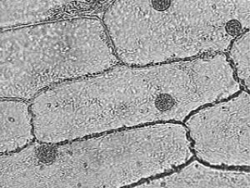
\includegraphics[width=\linewidth,keepaspectratio]{images/250px-Image005.png}} \\
    \caption{Onion cells in bright-field illumination. Round object in each cell is the nucleus. \\ \href{http://experimentationlab.berkeley.edu/sites/default/files/images/Rods_3450.JPG}\textbf{Click here to see larger picture}}
\end{minipage}\hfill
\begin{minipage}[h]{.49\linewidth}
    \centering
    \href{http://experimentationlab.berkeley.edu/sites/default/files/images/Image003.png}{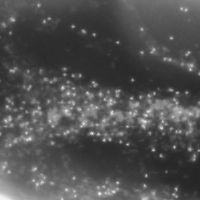
\includegraphics[width=\linewidth,keepaspectratio]{images/Image003.png}} \\
    \caption{Vesicles in the cytoplasm of a plant cell, as seen in dark-field. \\ \href{http://experimentationlab.berkeley.edu/sites/default/files/images/Rods_3450.JPG}\textbf{Click here to see larger picture}}
\end{minipage} 
\end{figure}

\begin{figure}
\begin{minipage}[h]{.49\linewidth}
    \centering
    \href{http://experimentationlab.berkeley.edu/sites/default/files/images/250px-Image005.png}{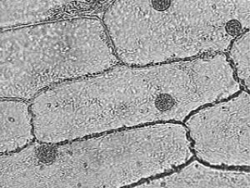
\includegraphics[width=\linewidth,keepaspectratio]{images/250px-Image005.png}} \\
    \caption{Onion cells in bright-field illumination. Round object in each cell is the nucleus. \\ \href{http://experimentationlab.berkeley.edu/sites/default/files/images/Rods_3450.JPG}\textbf{Click here to see larger picture}}
\end{minipage}\hfill
\begin{minipage}[h]{.49\linewidth}
    \centering
    \href{http://experimentationlab.berkeley.edu/sites/default/files/images/Image003.png}{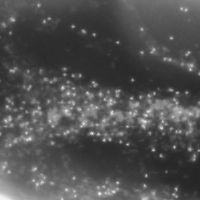
\includegraphics[width=\linewidth,keepaspectratio]{images/Image003.png}} \\
    \caption{Vesicles in the cytoplasm of a plant cell, as seen in dark-field. \\ \href{http://experimentationlab.berkeley.edu/sites/default/files/images/Rods_3450.JPG}\textbf{Click here to see larger picture}}
\end{minipage} 
\end{figure}

\noindent
\href{http://experimentationlab.berkeley.edu/sites/default/files/images/Rods_3450.JPG}{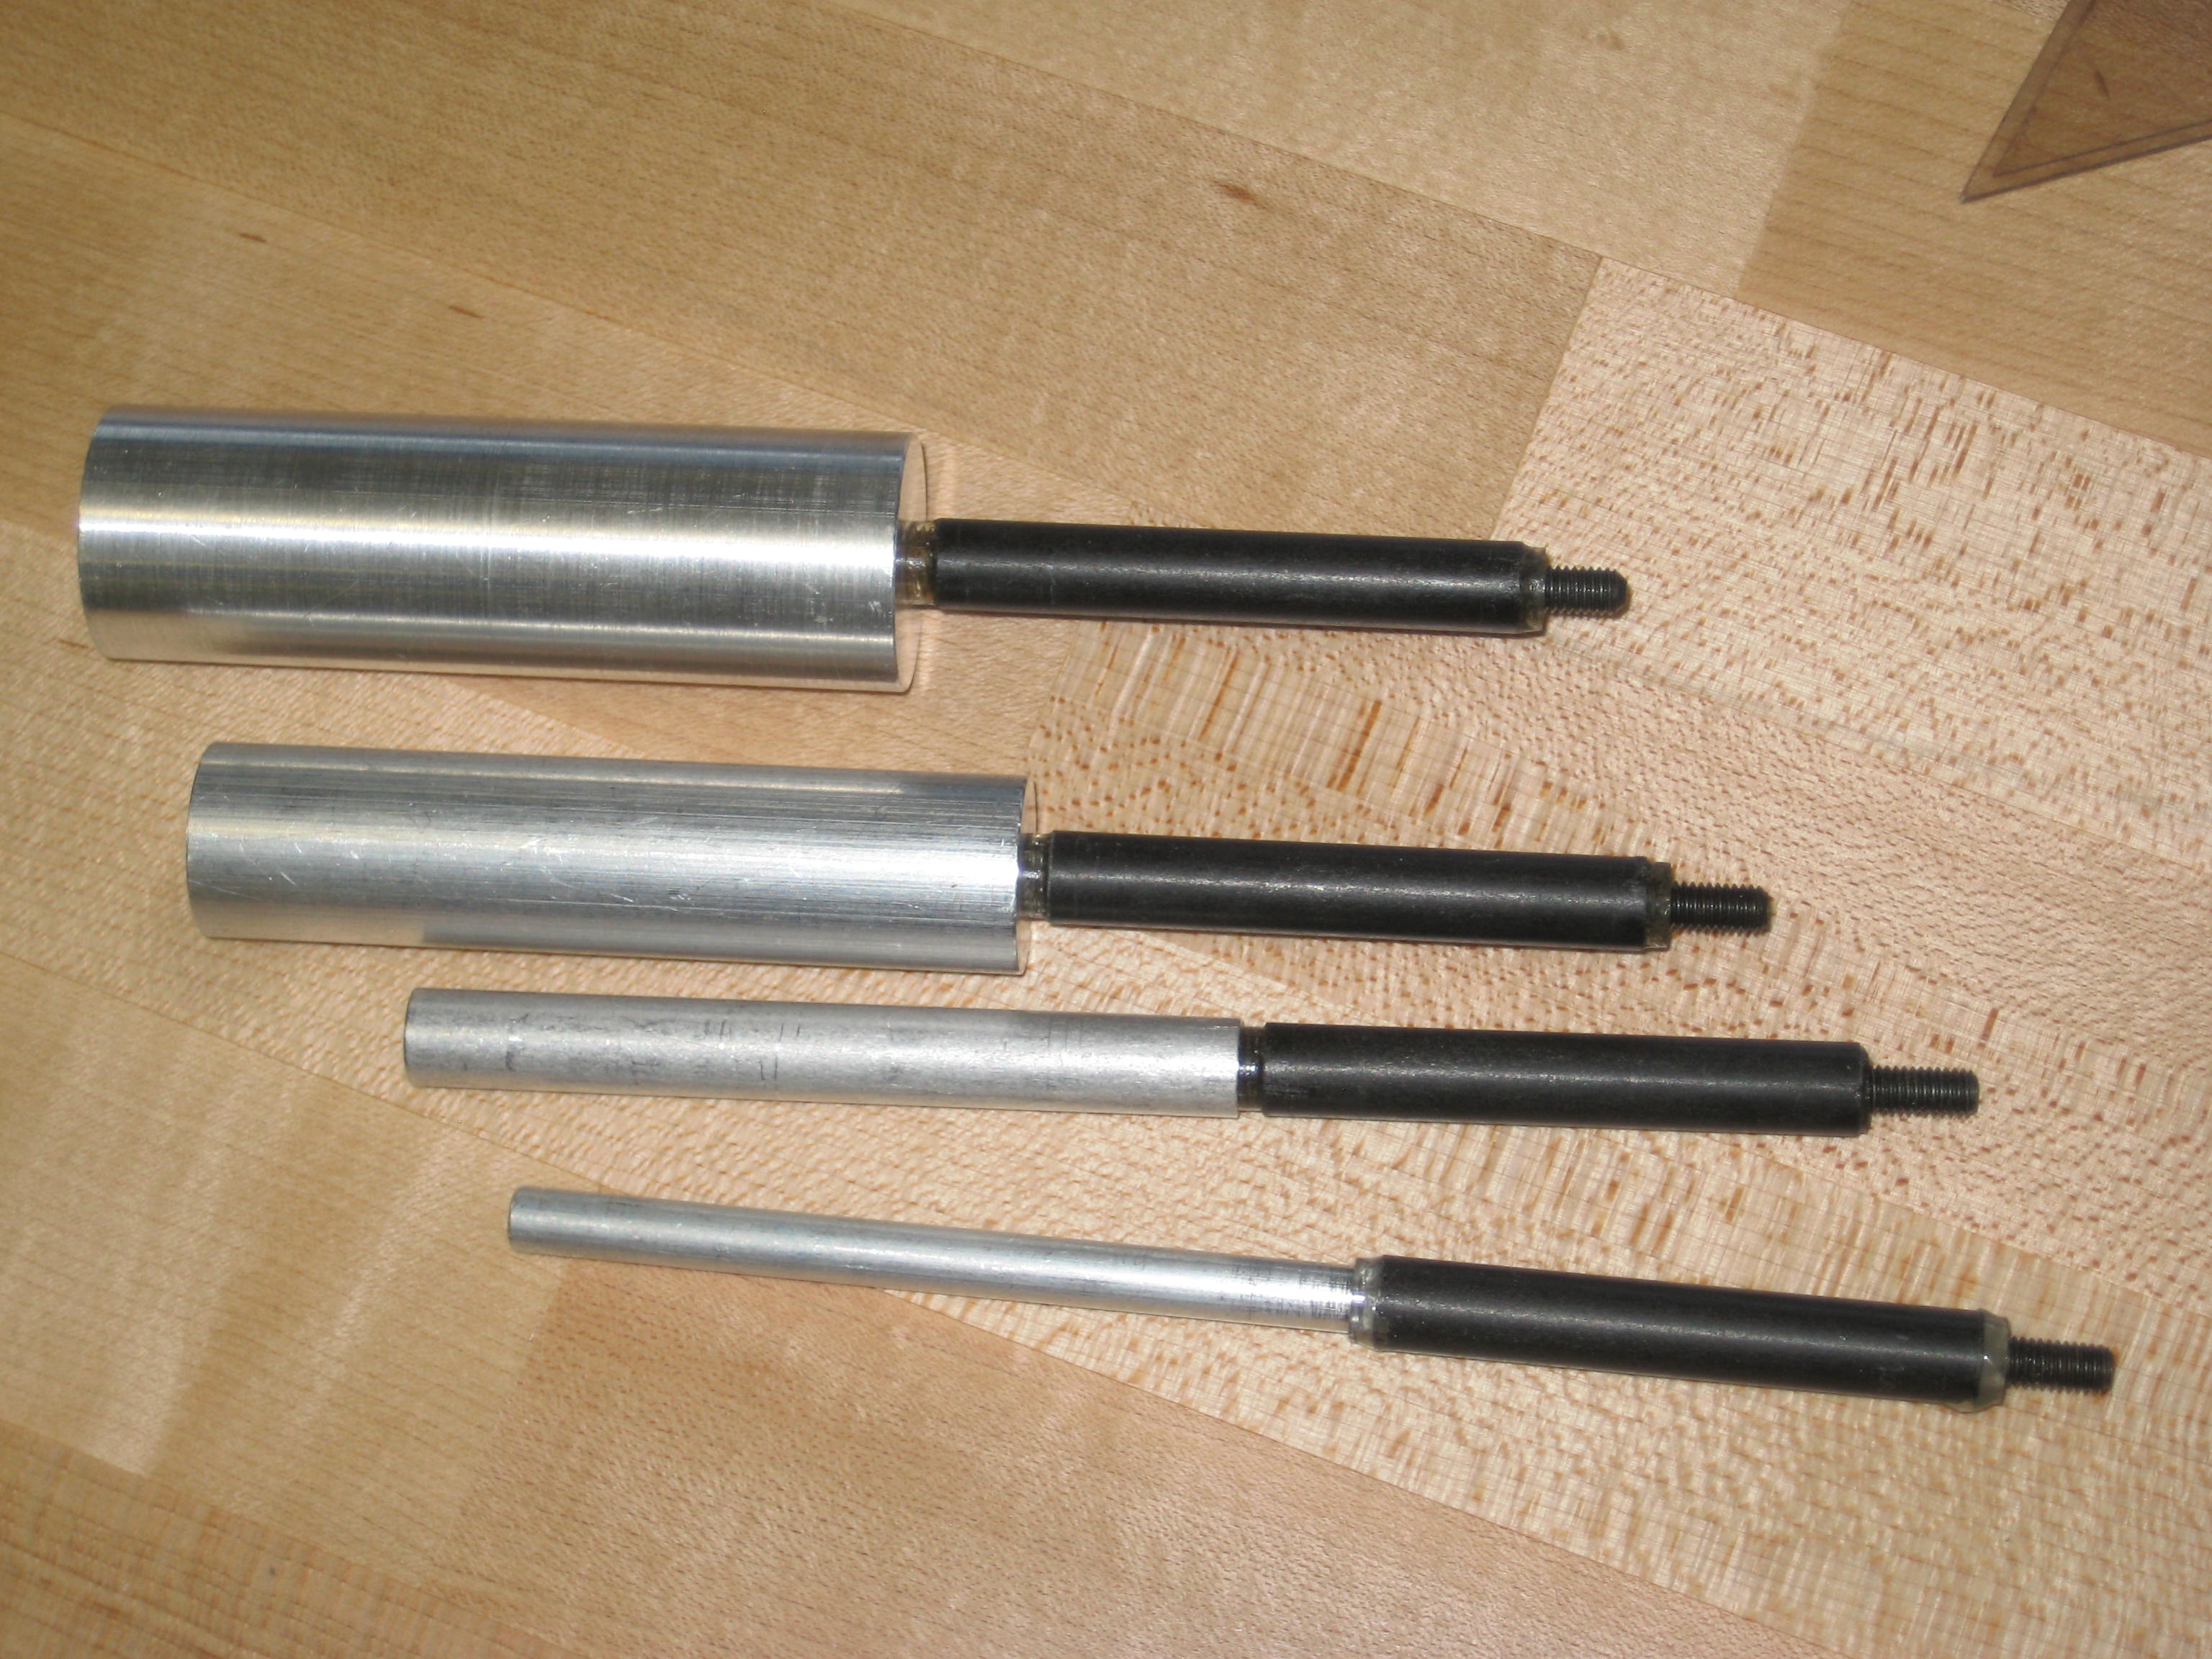
\includegraphics[width=0.33\linewidth,keepaspectratio]{images/Rods_3450.JPG}}
\href{http://experimentationlab.berkeley.edu/sites/default/files/images/COM_3.JPG}{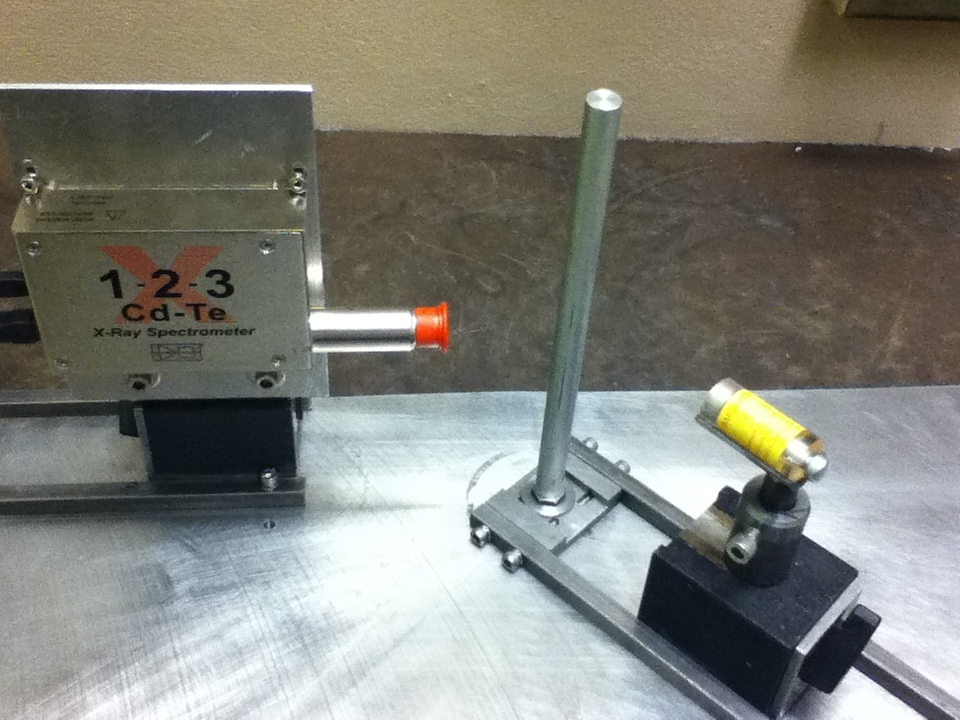
\includegraphics[width=0.33\linewidth,keepaspectratio]{images/COM_3.JPG}}
\href{http://experimentationlab.berkeley.edu/sites/default/files/images/COM_3526-Lg.JPG}{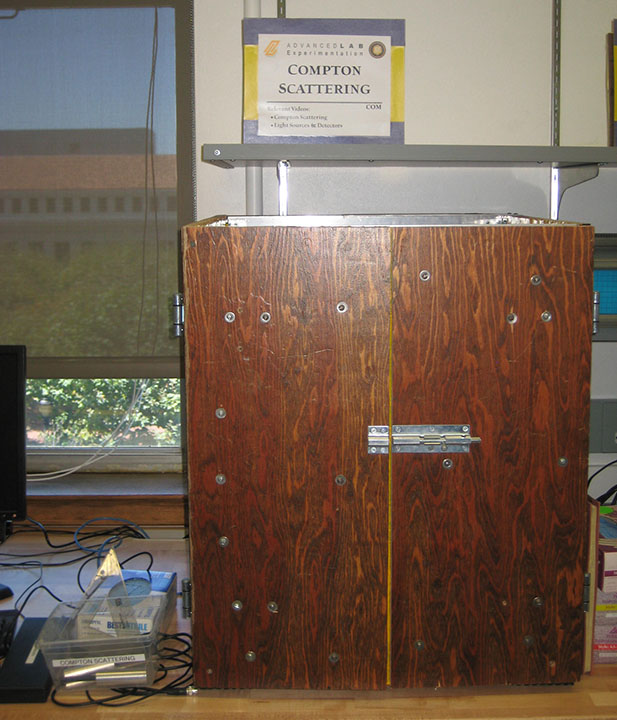
\includegraphics[width=0.33\linewidth,keepaspectratio]{images/COM_3526-Lg.JPG}}
\href{http://experimentationlab.berkeley.edu/sites/default/files/images/COM_Inside_3525-Lg.JPG}{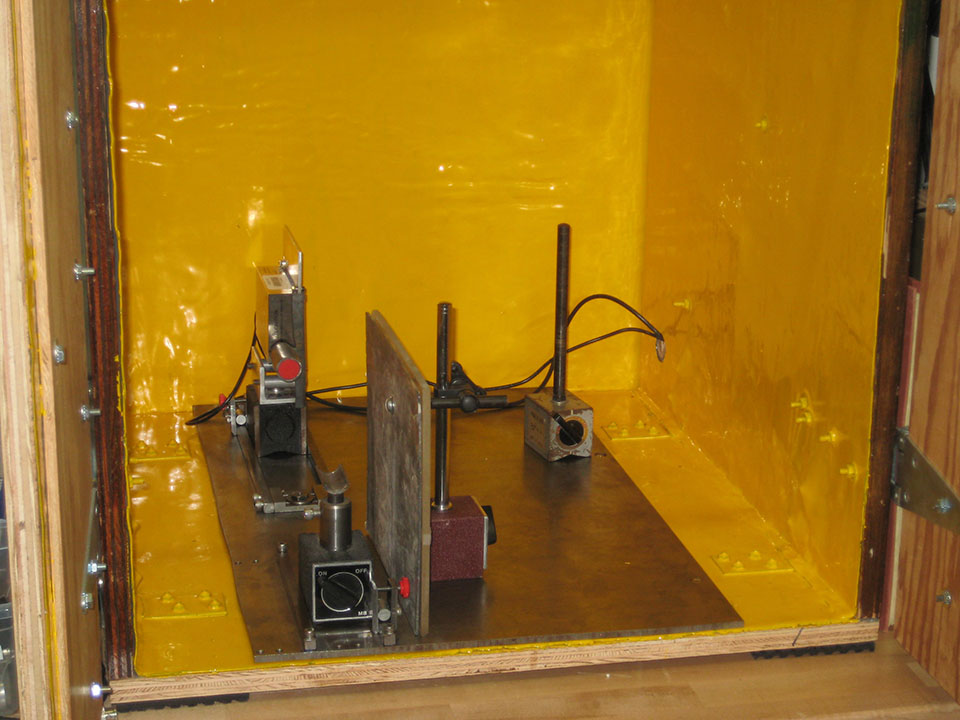
\includegraphics[width=0.33\linewidth,keepaspectratio]{images/COM_Inside_3525-Lg.JPG}}

\section{Before the 1st Day Lab and Standard Operating Procedure, SOP's for Compton}
\label{sec:BeforeTheLab}

\textbf{Complete the following before your experiment's scheduled start date:}

\begin{enumerate}
    \item View the \href{http://youtu.be/PVgqyf3kNRs}{\textbf{Compton Scattering video}} and \href{http://youtu.be/lQKLakISoBA}{\textbf{``Light Sources and Detectors'' video}}.

    \item \emph{Checkpoints are examination points where you must STOP and get a GSI or professor to verify your understanding and/or verify proper experimental setup. You cannot skip the checkpoints, as there is a \href{http://experimentationlab.berkeley.edu/node/132}{\textbf{sign off sheet}} that must be scanned in with your lab report. Print out the checkpoints page now and look it over.}

    \item View the     ``\href{http://youtu.be/KHxtzF5pZZM}{\textbf{Radiation Safety Video}}.'' After watching the video in the 111-Lab, get a pink Radiation Safety form from a 111-Lab staff person. Fill it out \& sign the form for getting a \textbf{Radiation Ring}.

    \item Now complete the Radiation Safety Training \href{http://experimentationlab.berkeley.edu/RadiationSafety}{\textbf{Radiation Safety}} \textbf{After completion of Training turn in all forms to Don Orlando.}

    \item Complete the \href{http://experimentationlab.berkeley.edu/COMPreLab}{\textbf{COM Pre Lab and Evaluation}} sheets. Print, fill it out, then turn in with your answers. The Pre-Lab must be printed separately. Discuss the experiment and pre-lab questions with any faculty member or GSI and get it signed off by that faculty member or GSI. Turn in the signed pre-lab sheet with your lab report.

    \item View the \href{\ErrorAnalysisVideo}{\textbf{Introduction to Error Analysis video}} and \href{\ErrorAnalysisNotes}{\textbf{\textbf{Error Analysis Notes}}}.

    \item Read the Standard Operating Procedures (SOP) for this lab before starting \href{http://experimentationlab.berkeley.edu/sites/default/files/images/SOP\_3271\_Cs-137\_Na-22\_Co-60\_Mn-54\_Am-241\_Fe-55\_2014.pdf}{\textbf{SOP\_3271\_Cs-137\_Na-22\_Co-60\_Mn-54\_Am-241\_Fe-55\_2014}}.

    \item Last day of the experiment please fill out the \href{\ExperimentEvaluation}{\textbf{Experiment Evaluation}}

\end{enumerate}

\textbf{Suggested Reading:}

\begin{itemize}
    \item Melissinos. \href{http://physics111.lib.berkeley.edu/Physics111/Reprints/COM/Melissinos\%201966\%20pg\%20252-265\%20and\%20369-384.pdf}{\textbf{``Compton Scattering'' pp. 252-265 and pp. 369-384}}; " \emph{Experiments in Modern Physics}, (Academic Press, 1966). \#QC33.M4 and or [pp. 369-384 in second ed.] \#QC33.M52

    \item DP5 .....\href{http://experimentationlab.berkeley.edu/sites/default/files/images/DP5\_Quick\_Start-Guide\_B0.pdf}{\textbf{Quick start Guide}}

\end{itemize}

\begin{enumerate}
    \item X-123 ....\href{http://experimentationlab.berkeley.edu/sites/default/files/images/X-123.pdf}{\textbf{X-123 Amplifier Detector Quick Start Guide}}

    \item Knoll, \emph{Radiation Detection and Measurement}, (Wiley, 1979).Ch.2,Ch.3, and Ch.10 for a good description of general detection principles, and semi-conductor detectors; and the ``Compton Effect'' article attached to this lab manual. \href{http://physics111.lib.berkeley.edu/Physics111/Reprints/COM/01-Radiation\_Detection\_and\_Measurement\_CH\_02.pdf}{\textbf{Ch.2 Radiation Interactions}},\href{http://physics111.lib.berkeley.edu/Physics111/Reprints/COM/01-Radiation\_Detection\_and\_Measurement\_CH\_03.pdf}{\textbf{Ch.3 General Radiation Detection}},\href{http://physics111.lib.berkeley.edu/Physics111/Reprints/COM/01-Radiation\_Detection\_and\_Measurement\_CH\_10.pdf}{\textbf{Ch.10 Radiation Spectroscopy with Scintillators}},\href{http://physics111.lib.berkeley.edu/Physics111/Reprints/COM/01-Radiation\_Detection\_and\_Measurement\_CH\_11.pdf}{\textbf{Ch.11 Semiconductor Detectors}}, and \href{http://physics111.lib.berkeley.edu/Physics111/Reprints/COM/Knoll\_ch.\%2012\%20lithium-drifted\%20germanium\%20detectors.pdf}{\textbf{Ch.12 SiLi Solid State Detectors}}

    \item \href{http://experimentationlab.berkeley.edu/sites/default/files/images/DP5\_User\_Manual\_A1.pdf}{\textbf{Dp5 User Manual}}

\end{enumerate}

More \hyperref[sec:References]{References}

[\href{\LabReprints}{\textbf{Physics 111 Library Site}}]

You should keep a laboratory notebook. The notebook should contain a detailed record of everything that was done and how/why it was done, as well as all of the data and analysis, also with plenty of how/why entries. This will aid you when you write your report.

\section{Objectives}

\begin{itemize}
    \item Learn about the Compton effect

    \item Learn the Klein-Nishina formula

    \item Learn about scattering cross section for quantum scattering

    \item Measure the mass of the electron

    \item Apply error analysis techniques to a data set that you collect

\end{itemize}

\section{Introduction}

The \emph{scattering of X-rays by electrons }was explored by A. H. Compton in the early part of the 20th century. The reduced frequency of the scattered photon is fundamental evidence for the proportionality of energy to the frequency of light, and for the relativistic kinematics of electrons. In 1929 Klein and Nishina calculated the \emph{angular distribution} of Compton scattering from free electrons in one of the first applications of quantum electrodynamics (QED). The Klein-Nishina gives the probability, the differential cross section, that a photon will be scattered into a given solid angle. Today, when applied to electromagnetic processes 50 million times more energetic, QED predictions still appear to be borne out.

Your goals for this lab are to observe and analyze Compton scattering and to learn something about semiconductor detectors. You will use your Compton scattering data to compare the observed energy shifts with the theoretical predictions, to determine the mass of the electron, and to attempt a verification of the Klein-Nishina formula.

\section{Theory}

The Compton scattering process consists of a photon scattering off of a (free) electron. The scattering formula is
\begin{equation}
    \lambda'-\lambda=\left ( \frac{h}{m_ec}\right)\left (1-\cos{\theta}\right )=\lambda_c(1-\cos{\theta})
\end{equation}
where $\lambda'$ is the wavelength of the scattered photon, $\lambda$ is the wavelength of the incident photon, $\theta$ is the scattering angle, and $\lambda_c$ is the Compton wavelength of the electron, equals to 2426 fermi ($2426 \times 10^{-15}$). By comparison, the wavelength of a 59.54 keV X-ray is 20824 Fm. You will need to convert the wavelength of the scattered photon into \emph{energy}, which is measured by the detector. You should derive the Compton formula, but do \emph{not} include it in your report. Rather, explain where it comes from, including any conservation laws and assumptions that are used.

The scattered X-ray energy may deviate from this prediction by roughly 1 part in 1000 if the electron from which it scatters is a bound valence electron. Can you explain why this is so?

\section{Apparatus}

All the apparatus comes packaged together in one box

\begin{enumerate}
    \item Amptek CdTe detector ($3 \times 3 \times 1$ mm$^{3}$).....\href{http://experimentationlab.berkeley.edu/sites/default/files/images/X-123\_CdTe\_User\_Manual.pdf}{\textbf{X-123\_CdTe\_User\_Manual}}

    \item Detector Pre-amplifier

    \item Digital pulse processor

    \item Detector and pre-amp power supply

\end{enumerate}

Other user Manuals and information on the X-123 Detector

\href{http://experimentationlab.berkeley.edu/sites/default/files/images/DP5\_Programmers\_Guide\_A4.pdf}{\textbf{DP5 Programmer's Guide}} \href{http://experimentationlab.berkeley.edu/sites/default/files/images/X-123.pdf}{\textbf{X-123 Amplifier Detector Quick Start Guide}}

\begin{itemize}
    \item \textbf{If you have any problems with the apparatus see Don Orlando}
\end{itemize}

\subsection{Source}

This experiment uses an $^{241}$Am (americium) at 130uCi radioactive source to provide the photons for scattering. The source is located in the lead box below the bench on the floor. Leave the source in the plastic box, in which it is contained. When working near the source, you must wear your radiation ring, and when handling the source you must wear vinyl gloves. Please remember to \emph{remove }the gloves before touching anything else or you will defeat the purpose of the gloves! Place the source at the height of the detector roughly 15cm away from the detector.

The source is made by placing a small amount of radioactive Am material inside an aluminum holder as shown. There is a lead backing behind the material that strongly attenuates the number of photons emitted at greater than 90 degrees in either direction of the source-end; radiation effectively is only emitted from the source-end (the side opposite the screw).

There is an energy level diagram of Am posted in the Compton experiment area. (There are more transitions possible than the strongest ones, which are listed below.)

\emph{Energies and branching fractions of X-rays from $^{241}$Am}

13.5 keV 12.8\%

17.3 keV 22.4\%

20.9 keV 6.2\%

26.3 keV 2.8\%

59.54 keV 40\%

\subsection{CdTe Detector}

\emph{The CdTe detector detects X-rays primarily by what means?} In your laboratory report you should briefly explain how the energies of the X-rays are registered by the detector and then converted into the voltage pulses that are accumulated by the multi channel analyzer (MCA). Note that while the detector is protected by a 1.5 cm cap, it is actually only 3 $\times$ 3 mm in size and 1 mm thick. It is placed behind the 100 $\mu$m thick Be window which sits 1.5 inches from the cap.

For information on the spectrometer system, see the \href{http://experimentationlab.berkeley.edu/sites/default/files/images/DP5\_User\_Manual\_A1.pdf}{\textbf{Dp5 User Manual}} and the book Knoll.

The X-ray detector is mounted on the 1.5 in extender and is coupled to a charge sensitive preamplifier. The output of the preamp is sent to the DP5 digital pulse processor which implements functions such as pulse shaping, pulse selection logic, pulse counters, a multichannel analyzer, and interfaces for data acquisition and control. The detector and preamp power supplies are housed together with the detector itself. It requires a +5VDC input and supplies the necessary voltages to the preamp.

\begin{figure}
    \centering
    \href{http://experimentationlab.berkeley.edu/sites/default/files/images/COMimage01.jpg}{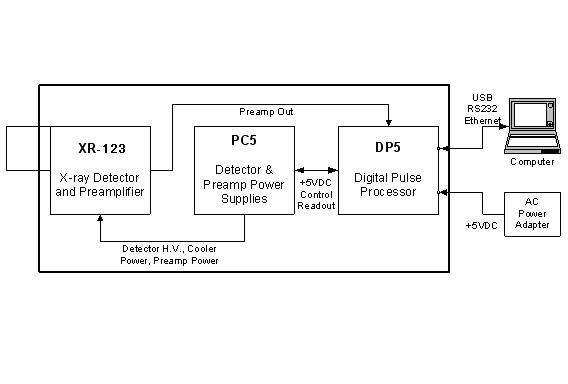
\includegraphics[width=0.7\linewidth]{images/COMimage01.jpg}}
    \caption{}
    \label{COMimage01}
\end{figure}

A photon striking the detector generates an output current pulse, which is turned into a voltage pulse and amplified by the pre-amp and amplifier systems. The DP5 digitizes the analog signal from the preamp, performs pulse shaping and pulse selection logic, determines the amplitude of the pulses and allocates this value to a histogram . The counts are binned in a channel corresponding to the detected energy. This produces the spectrum which is displayed on the computer. The Amptek ADMCA program allows you to choose from 256 to 8192 channels and the width of each channel will be approximately your full scale energy divided by the number of channels. In the experiment you should adjust the parameters so that you obtain an optimal full scale energy range. 

\textbf{Checkpoint: Why? What happens if your full scale energy range is too large or too small? How will you judge when you have obtained an appropriate range?}

It takes a finite amount of time for the PHA unit to sense a pulse, determine its height, place it in the proper channel, and then set up for sensing the next pulse. Pulses that arrive too closely together in time cannot be distinguished and yield problems with \emph{PHA Dead Time}. However, the rates for this experiment are low enough that this should not be a problem.

Understanding some basics of the DP5 digital pulse processor helps with optimizing the system configuration (that is, to get the best resolution for the energy peaks). See the manual for details. You might have to change some parameters for the pulse shaping, gain, thresholds, etc, to optimize your data acquisition. For example setting a low peaking time results in higher count rates attainable by the detector, but results in lower accuracy when determining the photon energies. A high peaking time does the opposite (lower count rates, more accuracy). However, for our Americium source, this rate is low enough that it is not necessary for us to use a low peaking time, and it is accurate enough that you don't need to use the high peaking times (otherwise it takes much longer to obtain usable data). [Note: As of July 2011, set the peaking time to 4.8 $\mu$s, flat top width to 0.2 $\mu$s, fast threshold to 25.] Again, you will find this information in the manual.

See \href{\ErrorAnalysisNotes}{\textbf{\textbf{Error Analysis Notes}}} for further computer information.

The detector electronics are already in place but may need to be connected; so check the cables. The equipment is easily damaged, expensive, and time-consuming to repair or replace. Thus, ask for help if you do not understand something!

Keep the following in mind:The red polyethylene safety cap should never be removed from the detector face!

\subsection{Scattering Apparatus}

The main components of the Apparatus consist of the $^{241}$Am source, the Amptek X-123 CdTe detector, and the five (5) aluminum rods of various sizes. Each rod is about 8-cm-long, and is screwed onto a low-mass rod that in turns can be screwed onto the steel plate base. \textbf{(Be careful not to over tighten the rods, you can break the low mass rods).} The detector and the source sit about 10.5 cm above the surface such that they are placed midway the height of the target. The $^{241}$Am source is removable and is kept in its plastic case inside a lead box when not in use. The source mounts on top of a steel holder which is held in place by a post on a magnetic base. The same goes for the detector. These bases can be secured in position by turning on/off the magnets that hold the bases to the steel surface. The detector mount can only be translated radially while the source may be displaced radially and rotated about the aluminum target. The surface of the set-up have markings which allow you to determine the scattering angle $\theta$.

\textbf{Checkpoint: Stop! Call a GSI over and demonstrate your understanding of the apparatus and all the appropriate safety procedures you will follow when dealing with it.}

\section{Standard Operating Procedure (SOP) for Seal Source experiment}

Before proceeding, see a staff member to obtain a radiation ring. The ring should be worn on whichever hand will be closer to the source.

\begin{enumerate}
    \item You should have completed the Radiation Safety Training above \hyperref[sec:BeforeTheLab]{Before the Lab}

    \item To start the detector you need to launch the ADMCA software by opening the ADMCA.exe file on the DeskTop and then connecting the PC to the detector by choosing DP5/X123-SDD in the dialog box. Clear any data that is saved from previous runs.

    \item Remove the $^{241}$Am source from the lead box on the floor, leaving it in its plastic case. Wear your radiation ring, and use the rubber gloves when handling the sources! Also, remember to \textbf{remove} the gloves before touching anything else or you will defeat the purpose of the gloves. Place the source on a stand at the height of the detector roughly 15 cm away from the detector.

    \item Calibrate your detector by taking a spectrum as shown below. That is, determine the relation between energy and channel numbers. Reference the known energies of the x-rays emitted by $^{241}$Am that are listed in the beginning of this write-up. Note: You can simply take a spectrum and use it to calibrate the detector, however, try to adjust your parameters so that you are taking advantage of the full range of channels. The Americium spectrum should look something that looks like this:
    \begin{figure}[h]
        \centering
        \href{http://experimentationlab.berkeley.edu/sites/default/files/images/550px-COMimage02.jpg}{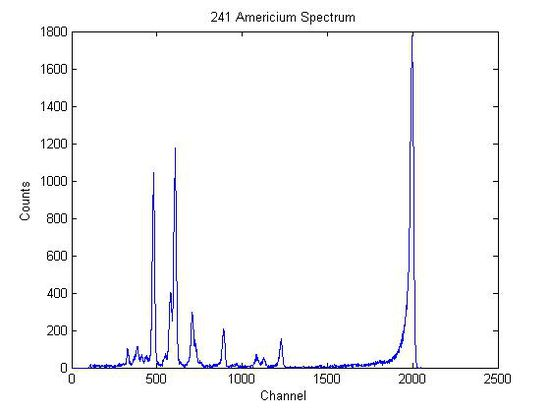
\includegraphics[width=0.8\linewidth]{images/550px-COMimage02.jpg}}
        \caption{$^{241}$Am source Energy Spectrum}
        \label{fig:550px-COMimage02}
    \end{figure}
 
	Determine the uncertainties in your fit parameters and the value of the reduced $x^2$. If you are missing the 59.54 keV peak (far right), your amplification/gain is probably too high. \emph{\textbf{Checkpoint: Make sure you can do the following/answer the following questions before calling over your GSI or Professor to sign you off:
	Show the staff your setup for calibration. Erase any existing data in the program (the button to the right of the little traffic light in the toolbar). The staff will verify that data collection is working properly.}}

    \item To observe Compton scattering you will want to use the 59.54 keV photons as they're the clearest to measure. When setting up your scattering apparatus keep in mind how the placement of the source, target, and detector affect your counting rate, resolution, background, etc. For example, you will have to place a small lead sheet between the source and detector to shield this from direct radiation from the source when you are interested in events coming from the target. Try using the different targets available; keep in mind that different targets introduce different factors which you will have to consider when measure the Compton scattering cross section for five different scattering angles. Note: you can see the peaks of the scattered photos for the smaller angles and higher angles in an afternoon (4 hours), but for other scattering angles you will need to leave the detector running after lab-hours; so plan accordingly. In general, longer runs at a given angle yield better data.

    \begin{itemize}
        \item After acquiring data for some scattering angles you should be able to answer questions 2 and 6 below, that is, measuring the FWHM of your peaks and say something about their broadness. Also, for scattering angles below around 100 degrees (depending on your set-up) you might observe the presence of a double-peak. To help you understand this and answer some of the questions below, set your experiment as if you were measuring Compton scattering at one of your angles, except this time remove the target and take a new acquisition. What you are doing here is measuring the background which will help you improve the data you have taken. Now, measure the numerical value of your background and explain the meaning of this value. \emph{Where is it coming from?} If you measure the background at some other angle, what do you observe? Make sure to get the counting rate of your background so you can make adjustments when you are reducing your actual data. As a suggestion, for each scattering angle, measure the background first, save and clear the data, then simply place the target in place (or vice versa) so that the only change in the environment is the placement/removal of the scatterer. In this way, you can get a decent background spectrum/count rate in one afternoon and then measure scattering from the rod overnight. To get you started, you can measure Compton scattering at a low angle for 2 hours, and then measure its background for the remaining 2 hours so you can see this in an afternoon. Using a program such as MATLAB will help you reduce the background from your actual spectra. Afterwards you will want to take advantage of longer acquisition times.

    \end{itemize}

    \item In your data analysis you will want to compare the number of photons scattered into the different scattering angles, to the numbers predicted by the Klein-Nishina formula (see figure 3) so be sure to keep a record of how long each run is, which scattering target you're using, the distance between source-target and target-detector, and an estimate of how much of the target is illuminated by the source after the lead-shielding is in place for every scattering angle. These values will be necessary to calculate quantities such as number of scattering centers and incident flux at the target (see \href{http://physics111.lib.berkeley.edu/Physics111/Reprints/COM/Melissinos\%201966\%20pg\%20252-265\%20and\%20369-384.pdf}{\textbf{Melissinos}} [\href{http://physics111.lib.berkeley.edu/Physics111/Reprints/COM/COM\_index.html}{\textbf{Reading Materials}}]. If you start a run and then leave the area, leave a sign saying ``Do Not Disturb'' along with your names and when you will return. No responsibility is assumed for equipment left running with no indication of when you will return; such equipment may be turned off by the staff. If you are doing an overnight run and do not have the equipment scheduled for the following day, you must come at the start of lab to collect your data unless you make other arrangements.

    \item Find the radiation flux at the source (to be used in the Klein-Nishina verification). To determine the flux, use a program such as ``Matlab'' to find the \emph{yield} (the number of 59.54 keV photons). NOTE: you simply cannot use the number in the bin that corresponds to 59.54 keV, why? Dividing the \emph{yield} by the amount of time it took to get the spectrum (i.e. 5 minutes) you can find the flux at the detector. You should be able to find the flux at the source using this number and the fact that you know the source target distance (See \href{http://physics111.lib.berkeley.edu/Physics111/Reprints/COM/Melissinos\%201966\%20pg\%20252-265\%20and\%20369-384.pdf}{\textbf{Melissinos}}, pp. 261-265 5 under [\href{http://physics111.lib.berkeley.edu/Physics111/Reprints/COM/COM\_index.html}{\textbf{Reading Materials}}]). \textbf{Checkpoint: Make sure you can do the following/answer the following questions before calling over your GSI or Professor to sign you off:
	Show your calculations and your reasoning for your result above (the radiation flux at the source).}

    \begin{figure}[h]
        \centering
        \href{http://experimentationlab.berkeley.edu/sites/default/files/images/550px-COMimage013.jpg}{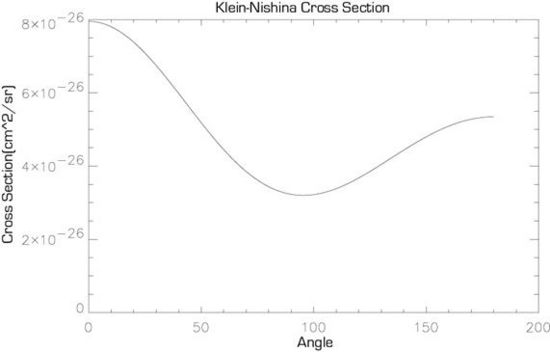
\includegraphics[width=0.7\linewidth]{images/550px-COMimage013.jpg}}
        \caption{Klein-Nishina Cross Section using Scattering Angles}
        \label{fig:550px-COMimage013}
    \end{figure}

    \item For something more complex, you will try to verify the Klein-Nishina formula for scattering within the detector, you need to run over the weekend so plan ahead. If we send monoenergetic X-rays directly into the detector without scattering them off of anything first, we should be able to observe Compton scattering off of the electrons within the detector. (See \emph{Knoll} [\href{http://physics111.lib.berkeley.edu/Physics111/Reprints/COM/COM\_index.html}{\textbf{Knoll}}]). For this effect to occur, the photon must enter the detector, scatter off of an electron, and then exit the detector. Since it is the electron energy that is ultimately processed to become the PHA count that we see, and since this electron energy is dependent upon the scattering angle, we should be able to see the Compton continuum predicted by Klein and Nishina (Figure 4). \emph{You should complete Questions} \emph{part 7 before you come to lab to begin taking the following data.} \textbf{Checkpoint: It's very important that you understand what is going on here before the weekend-long measurement. Give a GSI an overview of the physics involved in the experimental setup and your plan for the following measurement.} To obtain only 59.54 keV photons (eliminating the lower energy lines) that are unscattered before entering the detector, use the two brass plates with 1-mm aperture in the lead sheets for collimation and a brass plate with a 0.003``-thick Cu upstream of a 0.003''-thick Al sheet to filtering out the source X-rays with low energies. Align holes in the Brass collimator plates to be in line with the detector window. You will need to use these three plates and check the alignment of the holes to the detector. Measure the resulting spectrum by doing a long over-the-weekend run-you should see a continuum at lower energies that comes from Compton scattering off of the detector's own electrons as examined in \emph{\textbf{Questions}}, Part 7. The Klein-Nishina verification portion of this experiment does not work out as the model predicts. You should nevertheless try it, and put some thought into what might be going wrong. Do keep in mind that we are more concerned that you understand what it is that we are testing and what we expect (Questions, Part 7), than that you achieve ``the'' correct result. After all, in experimental physics it happens that something does not come out as expected at least as often as it does come out as expected. Examining and explaining these situations are often more worthwhile than looking at those in which the answers are already known.

    \begin{figure}[h]
        \centering
        \href{http://experimentationlab.berkeley.edu/sites/default/files/images/550px-COMimage014.jpg}{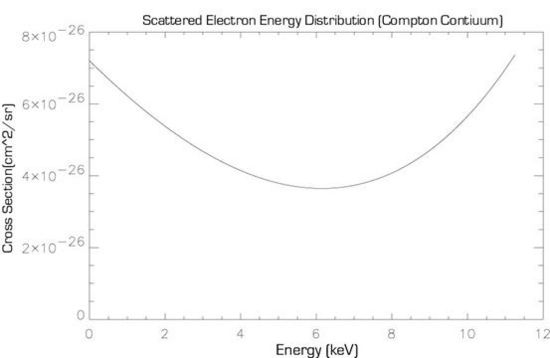
\includegraphics[width=0.7\linewidth]{images/550px-COMimage014.jpg}}
        \caption{Scattered Electron Energy Distribution using Compton Continuum}
        \label{fig:550px-COMimage014}
    \end{figure}

\end{enumerate}

\section{Questions}

\begin{enumerate}
    \item What accounts for the unshifted peaks that appear in your spectra taken at the different scattering angles? Can they be due to scattering off of the aluminum nuclei. (See Pre-lab questions.) (Hint: See \href{http://physics111.lib.berkeley.edu/Physics111/Reprints/COM/Melissinos\%201966\%20pg\%20252-265\%20and\%20369-384.pdf}{\textbf{Melissinos}}. [\href{http://physics111.lib.berkeley.edu/Physics111/Reprints/COM/COM\_index.html}{\textbf{Reading Materials}}])

    \item What is the full-width at half-maximum (FWHM) of each of your measured peaks of the $^{241}Am$ source, measured in energy, as listed in the section Source? How do these compare with the expected resolution of the detector? (See, for example, Knoll, pp. 89-92.)
    
    \item What is chi-square for the hypothesis that the X-ray energy and scattering angle are described by the Compton relationship?
    
    \item What is the value of the background (the contamination in the area of interest) that you measure? Why does it have this energy and where does it come from?
    
    \item How does the relative number of photons scattered into each scattering angle compare to the Klein-Nishina prediction? How about the Thomson cross section?
    
    \item Use your results from the scattering runs to determine the electron mass. What is the uncertainty in your value? Accuracy is optimized if the widest possible range of scattering angles is used.
    
    \item In the preceding question, you have assumed that the scattered beam was entirely monoenergetic. Is this actually true? Consider that there are several geometrical effects which cause the scattering angle to deviate from its nominal value-what are they, and how do they affect the results? This is not a trivial question! In particular, do they tend to shift your peaks from where you expect them to be, or do they tend to broaden the peaks about the expected value?
    
    \item In the last part of the lab you attempt to verify the Klein-Nishina prediction for Compton scattering within the detector. The theoretical prediction for this experiment consists of the following:
    \begin{enumerate}
        \item Prove that the scattered electron energy distribution $\frac{d\sigma}{dq'}$ and the scattered photon angular distribution $\frac{d\sigma}{d\Omega}$ are related by
        \begin{equation}
            \frac{d\sigma}{dq'}=\frac{d\sigma}{d\Omega}\frac{2\pi m_ec^2}{k'^2},
        \end{equation}
        where q' is the kinetic energy of the scattered electron and k' is the energy of the scattered photon. [\textbf{Hint}: note that
        \begin{equation}
            \frac{d\sigma}{dq'} = \frac{d\sigma}{d\Omega} \frac{d\Omega}{dq'} = \frac{d\sigma}{d\Omega} \left(\frac{dq'}{d\Omega} \right)^{-1},
        \end{equation}
        and recall that $d\Omega = 2 \pi \sin\theta d\theta$ since we have azimuthal symmetry.]
        
        \item The Klein-Nishina cross-section for scattering from a free electron is:
        \begin{equation}
            \frac{d\sigma}{d\Omega} = \frac{r_0^2}{2} \frac{f}{(1+g)^2} \left(1 + \frac{g^2}{f(1+g)}\right),
        \end{equation}
        where $r_0=\frac{e^2}{m_e c^2}$, the classical radius of the electron, and $f(\theta) = 1 + \cos^2 \theta$ and $g(\theta) = \frac{E_0}{m_ec^2} (1-\cos \theta)$,
        
        and $E_0$ = 59.54 keV for the $^{241}$Am photons that we use to observe Compton scattering.
        
        Make a plot of $\frac{d\sigma}{dq'}$ and include it in your report as the theoretical prediction for this part of the experiment.
    \end{enumerate}
    
\end{enumerate}

\begin{itemize}
    \item Last day of the experiment please fill out the \href{\ExperimentEvaluation}{\textbf{Experiment Evaluation}}

\end{itemize}

\section{References}
\label{sec:References}

\begin{enumerate}
    \item R. M. Eisberg et al., ``\href{http://physics111.lib.berkeley.edu/Physics111/Reprints/COM/Ch.\%203.8\%20The\%20compton\%20effect\%20pg\%2081-86.pdf}{\textbf{Chapter 3.8: The Compton Effect}} and \href{http://physics111.lib.berkeley.edu/Physics111/Reprints/COM/Ch.\%2014\%20X-rays.pdf}{\textbf{Chapter 14: X-Rays}}.'' \emph{Fundamentals of Modern Physics}, (Wiley, 1961), Physics Library Ref. QC173.E38.

    \item Gibson, ``\href{http://physics111.lib.berkeley.edu/Physics111/Reprints/COM/02-Semiconductor\_Particle\_Spectrometers.pdf}{\textbf{Semiconductor Particle Spectrometers}},'' from Siegbahn's \emph{Alpha-, Beta-, and Gamma-Ray Spectroscopy}. \#QC173.S536

    \item F. Goulding, ``\href{http://physics111.lib.berkeley.edu/Physics111/Reprints/COM/COM\_Detectors/01-UCRL-16231.pdf}{\textbf{Semiconductor Detectors for Nuclear Spectrometry}}.'' UCRL-16231

    \item Klein-Nishina formula: \href{http://physics111.lib.berkeley.edu/Physics111/Reprints/COM/Klein\_Nishina-Wiki.pdf}{\textbf{Wiki Klein-Nishina}}

    \item Other articles on Klein-Nishina \href{http://physics111.lib.berkeley.edu/Physics111/Reprints/COM/Klein\%20Nishina-p231\_1.pdf}{\textbf{PR-85-2-Jan.15,1952 Pg 231}}, \href{http://physics111.lib.berkeley.edu/Physics111/Reprints/COM/Klein\%20Nishina-p1975\_1.pdf}{\textbf{PR-185-5-Sept.25,1969 Pg 1975}}, \href{http://physics111.lib.berkeley.edu/Physics111/Reprints/COM/Klein\%20Nishina-p3061\_1.pdf}{\textbf{PRA-Vol27-6-June-1983 Pg 3061}} and \href{http://physics111.lib.berkeley.edu/Physics111/Reprints/COM/Klein\%20Nishina\_p75\_1.pdf}{\textbf{PRL-Vol10-3-1963 Pg 75}}

    \item Compton Detector Types: \href{http://physics111.lib.berkeley.edu/Physics111/Reprints/COM/COM\_index.html}{\textbf{Detectors}}

    \item R. D. Evans, \href{http://physics111.lib.berkeley.edu/Physics111/Reprints/R.D.Evans\%20Atomic\%20Nucleus/The\%20Atomic\%20Nucleus\%20Evans\%20full\%20text.pdf}{\textbf{The Atomic Nucleus}}, McGraw Hill (1972).

\end{enumerate}

Other reprints and reference materials can be found on the \href{http://physics111.lib.berkeley.edu/Physics111/Reprints/COM/COM\_index.html}{\textbf{Physics 111 Library Site}}

\end{document}